\documentclass{article}
\usepackage[utf8]{inputenc}

\usepackage[
backend=biber,
style=alphabetic,
sorting=ynt
]{biblatex}

\addbibresource{bibliography.bib}

\usepackage[english]{babel}
\usepackage{graphicx}
\usepackage{amssymb}
\usepackage[utf8]{inputenc}
\usepackage{fancyhdr}
\usepackage{natbib}
\usepackage{graphicx}
\usepackage{amssymb}
\usepackage{amsmath}
\usepackage{amsthm}
   \documentclass[11pt]{article}
   \newcommand{\norm}[1]{\left\lVert#1\right\rVert}

    \usepackage[breakable]{tcolorbox}
    \usepackage{parskip} % Stop auto-indenting (to mimic markdown behaviour)
    
    \usepackage{iftex}
    \ifPDFTeX
    	\usepackage[T1]{fontenc}
    	\usepackage{mathpazo}
    \else
    	\usepackage{fontspec}
    \fi

    % Basic figure setup, for now with no caption control since it's done
    % automatically by Pandoc (which extracts ![](path) syntax from Markdown).
    \usepackage{graphicx}
    % Maintain compatibility with old templates. Remove in nbconvert 6.0
    \let\Oldincludegraphics\includegraphics
    % Ensure that by default, figures have no caption (until we provide a
    % proper Figure object with a Caption API and a way to capture that
    % in the conversion process - todo).
    \usepackage{caption}
    \DeclareCaptionFormat{nocaption}{}
    \captionsetup{format=nocaption,aboveskip=0pt,belowskip=0pt}

    \usepackage[Export]{adjustbox} % Used to constrain images to a maximum size
    \adjustboxset{max size={0.9\linewidth}{0.9\paperheight}}
    \usepackage{float}
    \floatplacement{figure}{H} % forces figures to be placed at the correct location
    \usepackage{xcolor} % Allow colors to be defined
    \usepackage{enumerate} % Needed for markdown enumerations to work
    \usepackage{geometry} % Used to adjust the document margins
    \usepackage{amsmath} % Equations
    \usepackage{amssymb} % Equations
    \usepackage{textcomp} % defines textquotesingle
    % Hack from http://tex.stackexchange.com/a/47451/13684:
    \AtBeginDocument{%
        \def\PYZsq{\textquotesingle}% Upright quotes in Pygmentized code
    }
    \usepackage{upquote} % Upright quotes for verbatim code
    \usepackage{eurosym} % defines \euro
    \usepackage[mathletters]{ucs} % Extended unicode (utf-8) support
    \usepackage{fancyvrb} % verbatim replacement that allows latex
    \usepackage{grffile} % extends the file name processing of package graphics 
                         % to support a larger range
    \makeatletter % fix for grffile with XeLaTeX
    \def\Gread@@xetex#1{%
      \IfFileExists{"\Gin@base".bb}%
      {\Gread@eps{\Gin@base.bb}}%
      {\Gread@@xetex@aux#1}%
    }
    \makeatother

    % The hyperref package gives us a pdf with properly built
    % internal navigation ('pdf bookmarks' for the table of contents,
    % internal cross-reference links, web links for URLs, etc.)
    \usepackage{hyperref}
    % The default LaTeX title has an obnoxious amount of whitespace. By default,
    % titling removes some of it. It also provides customization options.
    \usepackage{titling}
    \usepackage{longtable} % longtable support required by pandoc >1.10
    \usepackage{booktabs}  % table support for pandoc > 1.12.2
    \usepackage[inline]{enumitem} % IRkernel/repr support (it uses the enumerate* environment)
    \usepackage[normalem]{ulem} % ulem is needed to support strikethroughs (\sout)
                                % normalem makes italics be italics, not underlines
    \usepackage{mathrsfs}
    

    
    % Colors for the hyperref package
    \definecolor{urlcolor}{rgb}{0,.145,.698}
    \definecolor{linkcolor}{rgb}{.71,0.21,0.01}
    \definecolor{citecolor}{rgb}{.12,.54,.11}

    % ANSI colors
    \definecolor{ansi-black}{HTML}{3E424D}
    \definecolor{ansi-black-intense}{HTML}{282C36}
    \definecolor{ansi-red}{HTML}{E75C58}
    \definecolor{ansi-red-intense}{HTML}{B22B31}
    \definecolor{ansi-green}{HTML}{00A250}
    \definecolor{ansi-green-intense}{HTML}{007427}
    \definecolor{ansi-yellow}{HTML}{DDB62B}
    \definecolor{ansi-yellow-intense}{HTML}{B27D12}
    \definecolor{ansi-blue}{HTML}{208FFB}
    \definecolor{ansi-blue-intense}{HTML}{0065CA}
    \definecolor{ansi-magenta}{HTML}{D160C4}
    \definecolor{ansi-magenta-intense}{HTML}{A03196}
    \definecolor{ansi-cyan}{HTML}{60C6C8}
    \definecolor{ansi-cyan-intense}{HTML}{258F8F}
    \definecolor{ansi-white}{HTML}{C5C1B4}
    \definecolor{ansi-white-intense}{HTML}{A1A6B2}
    \definecolor{ansi-default-inverse-fg}{HTML}{FFFFFF}
    \definecolor{ansi-default-inverse-bg}{HTML}{000000}

    % commands and environments needed by pandoc snippets
    % extracted from the output of `pandoc -s`
    \providecommand{\tightlist}{%
      \setlength{\itemsep}{0pt}\setlength{\parskip}{0pt}}
    \DefineVerbatimEnvironment{Highlighting}{Verbatim}{commandchars=\\\{\}}
    % Add ',fontsize=\small' for more characters per line
    \newenvironment{Shaded}{}{}
    \newcommand{\KeywordTok}[1]{\textcolor[rgb]{0.00,0.44,0.13}{\textbf{{#1}}}}
    \newcommand{\DataTypeTok}[1]{\textcolor[rgb]{0.56,0.13,0.00}{{#1}}}
    \newcommand{\DecValTok}[1]{\textcolor[rgb]{0.25,0.63,0.44}{{#1}}}
    \newcommand{\BaseNTok}[1]{\textcolor[rgb]{0.25,0.63,0.44}{{#1}}}
    \newcommand{\FloatTok}[1]{\textcolor[rgb]{0.25,0.63,0.44}{{#1}}}
    \newcommand{\CharTok}[1]{\textcolor[rgb]{0.25,0.44,0.63}{{#1}}}
    \newcommand{\StringTok}[1]{\textcolor[rgb]{0.25,0.44,0.63}{{#1}}}
    \newcommand{\CommentTok}[1]{\textcolor[rgb]{0.38,0.63,0.69}{\textit{{#1}}}}
    \newcommand{\OtherTok}[1]{\textcolor[rgb]{0.00,0.44,0.13}{{#1}}}
    \newcommand{\AlertTok}[1]{\textcolor[rgb]{1.00,0.00,0.00}{\textbf{{#1}}}}
    \newcommand{\FunctionTok}[1]{\textcolor[rgb]{0.02,0.16,0.49}{{#1}}}
    \newcommand{\RegionMarkerTok}[1]{{#1}}
    \newcommand{\ErrorTok}[1]{\textcolor[rgb]{1.00,0.00,0.00}{\textbf{{#1}}}}
    \newcommand{\NormalTok}[1]{{#1}}
    
    % Additional commands for more recent versions of Pandoc
    \newcommand{\ConstantTok}[1]{\textcolor[rgb]{0.53,0.00,0.00}{{#1}}}
    \newcommand{\SpecialCharTok}[1]{\textcolor[rgb]{0.25,0.44,0.63}{{#1}}}
    \newcommand{\VerbatimStringTok}[1]{\textcolor[rgb]{0.25,0.44,0.63}{{#1}}}
    \newcommand{\SpecialStringTok}[1]{\textcolor[rgb]{0.73,0.40,0.53}{{#1}}}
    \newcommand{\ImportTok}[1]{{#1}}
    \newcommand{\DocumentationTok}[1]{\textcolor[rgb]{0.73,0.13,0.13}{\textit{{#1}}}}
    \newcommand{\AnnotationTok}[1]{\textcolor[rgb]{0.38,0.63,0.69}{\textbf{\textit{{#1}}}}}
    \newcommand{\CommentVarTok}[1]{\textcolor[rgb]{0.38,0.63,0.69}{\textbf{\textit{{#1}}}}}
    \newcommand{\VariableTok}[1]{\textcolor[rgb]{0.10,0.09,0.49}{{#1}}}
    \newcommand{\ControlFlowTok}[1]{\textcolor[rgb]{0.00,0.44,0.13}{\textbf{{#1}}}}
    \newcommand{\OperatorTok}[1]{\textcolor[rgb]{0.40,0.40,0.40}{{#1}}}
    \newcommand{\BuiltInTok}[1]{{#1}}
    \newcommand{\ExtensionTok}[1]{{#1}}
    \newcommand{\PreprocessorTok}[1]{\textcolor[rgb]{0.74,0.48,0.00}{{#1}}}
    \newcommand{\AttributeTok}[1]{\textcolor[rgb]{0.49,0.56,0.16}{{#1}}}
    \newcommand{\InformationTok}[1]{\textcolor[rgb]{0.38,0.63,0.69}{\textbf{\textit{{#1}}}}}
    \newcommand{\WarningTok}[1]{\textcolor[rgb]{0.38,0.63,0.69}{\textbf{\textit{{#1}}}}}
    
    
    % Define a nice break command that doesn't care if a line doesn't already
    % exist.
    \def\br{\hspace*{\fill} \\* }
    % Math Jax compatibility definitions
    \def\gt{>}
    \def\lt{<}
    \let\Oldtex\TeX
    \let\Oldlatex\LaTeX
    \renewcommand{\TeX}{\textrm{\Oldtex}}
    \renewcommand{\LaTeX}{\textrm{\Oldlatex}}
    % Document parameters
    % Document title
    \title{FinalLinRegression}
    
    
    
    
    
% Pygments definitions
\makeatletter
\def\PY@reset{\let\PY@it=\relax \let\PY@bf=\relax%
    \let\PY@ul=\relax \let\PY@tc=\relax%
    \let\PY@bc=\relax \let\PY@ff=\relax}
\def\PY@tok#1{\csname PY@tok@#1\endcsname}
\def\PY@toks#1+{\ifx\relax#1\empty\else%
    \PY@tok{#1}\expandafter\PY@toks\fi}
\def\PY@do#1{\PY@bc{\PY@tc{\PY@ul{%
    \PY@it{\PY@bf{\PY@ff{#1}}}}}}}
\def\PY#1#2{\PY@reset\PY@toks#1+\relax+\PY@do{#2}}

\expandafter\def\csname PY@tok@w\endcsname{\def\PY@tc##1{\textcolor[rgb]{0.73,0.73,0.73}{##1}}}
\expandafter\def\csname PY@tok@c\endcsname{\let\PY@it=\textit\def\PY@tc##1{\textcolor[rgb]{0.25,0.50,0.50}{##1}}}
\expandafter\def\csname PY@tok@cp\endcsname{\def\PY@tc##1{\textcolor[rgb]{0.74,0.48,0.00}{##1}}}
\expandafter\def\csname PY@tok@k\endcsname{\let\PY@bf=\textbf\def\PY@tc##1{\textcolor[rgb]{0.00,0.50,0.00}{##1}}}
\expandafter\def\csname PY@tok@kp\endcsname{\def\PY@tc##1{\textcolor[rgb]{0.00,0.50,0.00}{##1}}}
\expandafter\def\csname PY@tok@kt\endcsname{\def\PY@tc##1{\textcolor[rgb]{0.69,0.00,0.25}{##1}}}
\expandafter\def\csname PY@tok@o\endcsname{\def\PY@tc##1{\textcolor[rgb]{0.40,0.40,0.40}{##1}}}
\expandafter\def\csname PY@tok@ow\endcsname{\let\PY@bf=\textbf\def\PY@tc##1{\textcolor[rgb]{0.67,0.13,1.00}{##1}}}
\expandafter\def\csname PY@tok@nb\endcsname{\def\PY@tc##1{\textcolor[rgb]{0.00,0.50,0.00}{##1}}}
\expandafter\def\csname PY@tok@nf\endcsname{\def\PY@tc##1{\textcolor[rgb]{0.00,0.00,1.00}{##1}}}
\expandafter\def\csname PY@tok@nc\endcsname{\let\PY@bf=\textbf\def\PY@tc##1{\textcolor[rgb]{0.00,0.00,1.00}{##1}}}
\expandafter\def\csname PY@tok@nn\endcsname{\let\PY@bf=\textbf\def\PY@tc##1{\textcolor[rgb]{0.00,0.00,1.00}{##1}}}
\expandafter\def\csname PY@tok@ne\endcsname{\let\PY@bf=\textbf\def\PY@tc##1{\textcolor[rgb]{0.82,0.25,0.23}{##1}}}
\expandafter\def\csname PY@tok@nv\endcsname{\def\PY@tc##1{\textcolor[rgb]{0.10,0.09,0.49}{##1}}}
\expandafter\def\csname PY@tok@no\endcsname{\def\PY@tc##1{\textcolor[rgb]{0.53,0.00,0.00}{##1}}}
\expandafter\def\csname PY@tok@nl\endcsname{\def\PY@tc##1{\textcolor[rgb]{0.63,0.63,0.00}{##1}}}
\expandafter\def\csname PY@tok@ni\endcsname{\let\PY@bf=\textbf\def\PY@tc##1{\textcolor[rgb]{0.60,0.60,0.60}{##1}}}
\expandafter\def\csname PY@tok@na\endcsname{\def\PY@tc##1{\textcolor[rgb]{0.49,0.56,0.16}{##1}}}
\expandafter\def\csname PY@tok@nt\endcsname{\let\PY@bf=\textbf\def\PY@tc##1{\textcolor[rgb]{0.00,0.50,0.00}{##1}}}
\expandafter\def\csname PY@tok@nd\endcsname{\def\PY@tc##1{\textcolor[rgb]{0.67,0.13,1.00}{##1}}}
\expandafter\def\csname PY@tok@s\endcsname{\def\PY@tc##1{\textcolor[rgb]{0.73,0.13,0.13}{##1}}}
\expandafter\def\csname PY@tok@sd\endcsname{\let\PY@it=\textit\def\PY@tc##1{\textcolor[rgb]{0.73,0.13,0.13}{##1}}}
\expandafter\def\csname PY@tok@si\endcsname{\let\PY@bf=\textbf\def\PY@tc##1{\textcolor[rgb]{0.73,0.40,0.53}{##1}}}
\expandafter\def\csname PY@tok@se\endcsname{\let\PY@bf=\textbf\def\PY@tc##1{\textcolor[rgb]{0.73,0.40,0.13}{##1}}}
\expandafter\def\csname PY@tok@sr\endcsname{\def\PY@tc##1{\textcolor[rgb]{0.73,0.40,0.53}{##1}}}
\expandafter\def\csname PY@tok@ss\endcsname{\def\PY@tc##1{\textcolor[rgb]{0.10,0.09,0.49}{##1}}}
\expandafter\def\csname PY@tok@sx\endcsname{\def\PY@tc##1{\textcolor[rgb]{0.00,0.50,0.00}{##1}}}
\expandafter\def\csname PY@tok@m\endcsname{\def\PY@tc##1{\textcolor[rgb]{0.40,0.40,0.40}{##1}}}
\expandafter\def\csname PY@tok@gh\endcsname{\let\PY@bf=\textbf\def\PY@tc##1{\textcolor[rgb]{0.00,0.00,0.50}{##1}}}
\expandafter\def\csname PY@tok@gu\endcsname{\let\PY@bf=\textbf\def\PY@tc##1{\textcolor[rgb]{0.50,0.00,0.50}{##1}}}
\expandafter\def\csname PY@tok@gd\endcsname{\def\PY@tc##1{\textcolor[rgb]{0.63,0.00,0.00}{##1}}}
\expandafter\def\csname PY@tok@gi\endcsname{\def\PY@tc##1{\textcolor[rgb]{0.00,0.63,0.00}{##1}}}
\expandafter\def\csname PY@tok@gr\endcsname{\def\PY@tc##1{\textcolor[rgb]{1.00,0.00,0.00}{##1}}}
\expandafter\def\csname PY@tok@ge\endcsname{\let\PY@it=\textit}
\expandafter\def\csname PY@tok@gs\endcsname{\let\PY@bf=\textbf}
\expandafter\def\csname PY@tok@gp\endcsname{\let\PY@bf=\textbf\def\PY@tc##1{\textcolor[rgb]{0.00,0.00,0.50}{##1}}}
\expandafter\def\csname PY@tok@go\endcsname{\def\PY@tc##1{\textcolor[rgb]{0.53,0.53,0.53}{##1}}}
\expandafter\def\csname PY@tok@gt\endcsname{\def\PY@tc##1{\textcolor[rgb]{0.00,0.27,0.87}{##1}}}
\expandafter\def\csname PY@tok@err\endcsname{\def\PY@bc##1{\setlength{\fboxsep}{0pt}\fcolorbox[rgb]{1.00,0.00,0.00}{1,1,1}{\strut ##1}}}
\expandafter\def\csname PY@tok@kc\endcsname{\let\PY@bf=\textbf\def\PY@tc##1{\textcolor[rgb]{0.00,0.50,0.00}{##1}}}
\expandafter\def\csname PY@tok@kd\endcsname{\let\PY@bf=\textbf\def\PY@tc##1{\textcolor[rgb]{0.00,0.50,0.00}{##1}}}
\expandafter\def\csname PY@tok@kn\endcsname{\let\PY@bf=\textbf\def\PY@tc##1{\textcolor[rgb]{0.00,0.50,0.00}{##1}}}
\expandafter\def\csname PY@tok@kr\endcsname{\let\PY@bf=\textbf\def\PY@tc##1{\textcolor[rgb]{0.00,0.50,0.00}{##1}}}
\expandafter\def\csname PY@tok@bp\endcsname{\def\PY@tc##1{\textcolor[rgb]{0.00,0.50,0.00}{##1}}}
\expandafter\def\csname PY@tok@fm\endcsname{\def\PY@tc##1{\textcolor[rgb]{0.00,0.00,1.00}{##1}}}
\expandafter\def\csname PY@tok@vc\endcsname{\def\PY@tc##1{\textcolor[rgb]{0.10,0.09,0.49}{##1}}}
\expandafter\def\csname PY@tok@vg\endcsname{\def\PY@tc##1{\textcolor[rgb]{0.10,0.09,0.49}{##1}}}
\expandafter\def\csname PY@tok@vi\endcsname{\def\PY@tc##1{\textcolor[rgb]{0.10,0.09,0.49}{##1}}}
\expandafter\def\csname PY@tok@vm\endcsname{\def\PY@tc##1{\textcolor[rgb]{0.10,0.09,0.49}{##1}}}
\expandafter\def\csname PY@tok@sa\endcsname{\def\PY@tc##1{\textcolor[rgb]{0.73,0.13,0.13}{##1}}}
\expandafter\def\csname PY@tok@sb\endcsname{\def\PY@tc##1{\textcolor[rgb]{0.73,0.13,0.13}{##1}}}
\expandafter\def\csname PY@tok@sc\endcsname{\def\PY@tc##1{\textcolor[rgb]{0.73,0.13,0.13}{##1}}}
\expandafter\def\csname PY@tok@dl\endcsname{\def\PY@tc##1{\textcolor[rgb]{0.73,0.13,0.13}{##1}}}
\expandafter\def\csname PY@tok@s2\endcsname{\def\PY@tc##1{\textcolor[rgb]{0.73,0.13,0.13}{##1}}}
\expandafter\def\csname PY@tok@sh\endcsname{\def\PY@tc##1{\textcolor[rgb]{0.73,0.13,0.13}{##1}}}
\expandafter\def\csname PY@tok@s1\endcsname{\def\PY@tc##1{\textcolor[rgb]{0.73,0.13,0.13}{##1}}}
\expandafter\def\csname PY@tok@mb\endcsname{\def\PY@tc##1{\textcolor[rgb]{0.40,0.40,0.40}{##1}}}
\expandafter\def\csname PY@tok@mf\endcsname{\def\PY@tc##1{\textcolor[rgb]{0.40,0.40,0.40}{##1}}}
\expandafter\def\csname PY@tok@mh\endcsname{\def\PY@tc##1{\textcolor[rgb]{0.40,0.40,0.40}{##1}}}
\expandafter\def\csname PY@tok@mi\endcsname{\def\PY@tc##1{\textcolor[rgb]{0.40,0.40,0.40}{##1}}}
\expandafter\def\csname PY@tok@il\endcsname{\def\PY@tc##1{\textcolor[rgb]{0.40,0.40,0.40}{##1}}}
\expandafter\def\csname PY@tok@mo\endcsname{\def\PY@tc##1{\textcolor[rgb]{0.40,0.40,0.40}{##1}}}
\expandafter\def\csname PY@tok@ch\endcsname{\let\PY@it=\textit\def\PY@tc##1{\textcolor[rgb]{0.25,0.50,0.50}{##1}}}
\expandafter\def\csname PY@tok@cm\endcsname{\let\PY@it=\textit\def\PY@tc##1{\textcolor[rgb]{0.25,0.50,0.50}{##1}}}
\expandafter\def\csname PY@tok@cpf\endcsname{\let\PY@it=\textit\def\PY@tc##1{\textcolor[rgb]{0.25,0.50,0.50}{##1}}}
\expandafter\def\csname PY@tok@c1\endcsname{\let\PY@it=\textit\def\PY@tc##1{\textcolor[rgb]{0.25,0.50,0.50}{##1}}}
\expandafter\def\csname PY@tok@cs\endcsname{\let\PY@it=\textit\def\PY@tc##1{\textcolor[rgb]{0.25,0.50,0.50}{##1}}}

\def\PYZbs{\char`\\}
\def\PYZus{\char`\_}
\def\PYZob{\char`\{}
\def\PYZcb{\char`\}}
\def\PYZca{\char`\^}
\def\PYZam{\char`\&}
\def\PYZlt{\char`\<}
\def\PYZgt{\char`\>}
\def\PYZsh{\char`\#}
\def\PYZpc{\char`\%}
\def\PYZdl{\char`\$}
\def\PYZhy{\char`\-}
\def\PYZsq{\char`\'}
\def\PYZdq{\char`\"}
\def\PYZti{\char`\~}
% for compatibility with earlier versions
\def\PYZat{@}
\def\PYZlb{[}
\def\PYZrb{]}
\makeatother


    % For linebreaks inside Verbatim environment from package fancyvrb. 
    \makeatletter
        \newbox\Wrappedcontinuationbox 
        \newbox\Wrappedvisiblespacebox 
        \newcommand*\Wrappedvisiblespace {\textcolor{red}{\textvisiblespace}} 
        \newcommand*\Wrappedcontinuationsymbol {\textcolor{red}{\llap{\tiny$\m@th\hookrightarrow$}}} 
        \newcommand*\Wrappedcontinuationindent {3ex } 
        \newcommand*\Wrappedafterbreak {\kern\Wrappedcontinuationindent\copy\Wrappedcontinuationbox} 
        % Take advantage of the already applied Pygments mark-up to insert 
        % potential linebreaks for TeX processing. 
        %        {, <, #, %, $, ' and ": go to next line. 
        %        _, }, ^, &, >, - and ~: stay at end of broken line. 
        % Use of \textquotesingle for straight quote. 
        \newcommand*\Wrappedbreaksatspecials {% 
            \def\PYGZus{\discretionary{\char`\_}{\Wrappedafterbreak}{\char`\_}}% 
            \def\PYGZob{\discretionary{}{\Wrappedafterbreak\char`\{}{\char`\{}}% 
            \def\PYGZcb{\discretionary{\char`\}}{\Wrappedafterbreak}{\char`\}}}% 
            \def\PYGZca{\discretionary{\char`\^}{\Wrappedafterbreak}{\char`\^}}% 
            \def\PYGZam{\discretionary{\char`\&}{\Wrappedafterbreak}{\char`\&}}% 
            \def\PYGZlt{\discretionary{}{\Wrappedafterbreak\char`\<}{\char`\<}}% 
            \def\PYGZgt{\discretionary{\char`\>}{\Wrappedafterbreak}{\char`\>}}% 
            \def\PYGZsh{\discretionary{}{\Wrappedafterbreak\char`\#}{\char`\#}}% 
            \def\PYGZpc{\discretionary{}{\Wrappedafterbreak\char`\%}{\char`\%}}% 
            \def\PYGZdl{\discretionary{}{\Wrappedafterbreak\char`\$}{\char`\$}}% 
            \def\PYGZhy{\discretionary{\char`\-}{\Wrappedafterbreak}{\char`\-}}% 
            \def\PYGZsq{\discretionary{}{\Wrappedafterbreak\textquotesingle}{\textquotesingle}}% 
            \def\PYGZdq{\discretionary{}{\Wrappedafterbreak\char`\"}{\char`\"}}% 
            \def\PYGZti{\discretionary{\char`\~}{\Wrappedafterbreak}{\char`\~}}% 
        } 
        % Some characters . , ; ? ! / are not pygmentized. 
        % This macro makes them "active" and they will insert potential linebreaks 
        \newcommand*\Wrappedbreaksatpunct {% 
            \lccode`\~`\.\lowercase{\def~}{\discretionary{\hbox{\char`\.}}{\Wrappedafterbreak}{\hbox{\char`\.}}}% 
            \lccode`\~`\,\lowercase{\def~}{\discretionary{\hbox{\char`\,}}{\Wrappedafterbreak}{\hbox{\char`\,}}}% 
            \lccode`\~`\;\lowercase{\def~}{\discretionary{\hbox{\char`\;}}{\Wrappedafterbreak}{\hbox{\char`\;}}}% 
            \lccode`\~`\:\lowercase{\def~}{\discretionary{\hbox{\char`\:}}{\Wrappedafterbreak}{\hbox{\char`\:}}}% 
            \lccode`\~`\?\lowercase{\def~}{\discretionary{\hbox{\char`\?}}{\Wrappedafterbreak}{\hbox{\char`\?}}}% 
            \lccode`\~`\!\lowercase{\def~}{\discretionary{\hbox{\char`\!}}{\Wrappedafterbreak}{\hbox{\char`\!}}}% 
            \lccode`\~`\/\lowercase{\def~}{\discretionary{\hbox{\char`\/}}{\Wrappedafterbreak}{\hbox{\char`\/}}}% 
            \catcode`\.\active
            \catcode`\,\active 
            \catcode`\;\active
            \catcode`\:\active
            \catcode`\?\active
            \catcode`\!\active
            \catcode`\/\active 
            \lccode`\~`\~ 	
        }
    \makeatother

    \let\OriginalVerbatim=\Verbatim
    \makeatletter
    \renewcommand{\Verbatim}[1][1]{%
        %\parskip\z@skip
        \sbox\Wrappedcontinuationbox {\Wrappedcontinuationsymbol}%
        \sbox\Wrappedvisiblespacebox {\FV@SetupFont\Wrappedvisiblespace}%
        \def\FancyVerbFormatLine ##1{\hsize\linewidth
            \vtop{\raggedright\hyphenpenalty\z@\exhyphenpenalty\z@
                \doublehyphendemerits\z@\finalhyphendemerits\z@
                \strut ##1\strut}%
        }%
        % If the linebreak is at a space, the latter will be displayed as visible
        % space at end of first line, and a continuation symbol starts next line.
        % Stretch/shrink are however usually zero for typewriter font.
        \def\FV@Space {%
            \nobreak\hskip\z@ plus\fontdimen3\font minus\fontdimen4\font
            \discretionary{\copy\Wrappedvisiblespacebox}{\Wrappedafterbreak}
            {\kern\fontdimen2\font}%
        }%
        
        % Allow breaks at special characters using \PYG... macros.
        \Wrappedbreaksatspecials
        % Breaks at punctuation characters . , ; ? ! and / need catcode=\active 	
        \OriginalVerbatim[#1,codes*=\Wrappedbreaksatpunct]%
    }
    \makeatother

    % Exact colors from NB
    \definecolor{incolor}{HTML}{303F9F}
    \definecolor{outcolor}{HTML}{D84315}
    \definecolor{cellborder}{HTML}{CFCFCF}
    \definecolor{cellbackground}{HTML}{F7F7F7}
    
    % prompt
    \makeatletter
    \newcommand{\boxspacing}{\kern\kvtcb@left@rule\kern\kvtcb@boxsep}
    \makeatother
    \newcommand{\prompt}[4]{
        \ttfamily\llap{{\color{#2}[#3]:\hspace{3pt}#4}}\vspace{-\baselineskip}
    }
    

    
    % Prevent overflowing lines due to hard-to-break entities
    \sloppy 
    % Setup hyperref package
    \hypersetup{
      breaklinks=true,  % so long urls are correctly broken across lines
      colorlinks=true,
      urlcolor=urlcolor,
      linkcolor=linkcolor,
      citecolor=citecolor,
      }
    % Slightly bigger margins than the latex defaults
    
    \geometry{verbose,tmargin=1in,bmargin=1in,lmargin=1in,rmargin=1in}
    
    

    
    
    % Define a nice break command that doesn't care if a line doesn't already
    % exist.
    \def\br{\hspace*{\fill} \\* }
    % Math Jax compatibility definitions
    \def\gt{>}
    \def\lt{<}
    \let\Oldtex\TeX
    \let\Oldlatex\LaTeX
    \renewcommand{\TeX}{\textrm{\Oldtex}}
    \renewcommand{\LaTeX}{\textrm{\Oldlatex}}
\begin{document}
\begin{titlepage}
   \begin{center}
       \vspace*{1cm}

       \huge \textbf{Mathematics for Machine Learning}

       \vspace{0.5cm}
        
            
       \vspace{1.5cm}

      
      \large \textbf{Aditya Reddy, Claire Guo, and Cole Wasserman}

      \vspace{35 mm}
            
       Final Project for Discrete Mathematics\\
            
       \vspace{0.8cm}
     
       
\includegraphics[width=0.4\textwidth]{university}
        \vspace{20 mm}     
       
       New York University\\
       Professor Normand\\
       December 2020\
            
   \end{center}
\end{titlepage}

\pagestyle{fancy}
\fancyhf{}
%\rhead{Aditya Reddy, Claire Guo, and Cole Wasserman}
\lhead{Mathematics for Machine Learning}
\rfoot{Page \thepage}
\tableofcontents
\newpage

\section{Abstract}

Machine learning is the process of mimicking human-like intuition through the capabilities of computer algorithms and the ability for machines to improve themselves through experience. Its applications are demonstrated through things such as data modeling, image/speech recognition, web recommendations/advertisements, etc. Unlike humans, who are able to see a given problem and instinctively produce a solution or method of solving the problem using our previous knowledge of what has worked and what has not, machines don’t have this capability; instead, they are only able to do exactly as dictated in the algorithms that we provide them with. However, the benefit of this is that machines are significantly faster at performing repeated tasks than humans are. Take the problem of finding the sum of $1+2+3+\dots+100$ for example. While there is obviously a formula to help us solve this problem faster, even applying it may take us a minute or so. A machine, however, given the correct code, would be able to find the solution in a fraction of a second, even by the method of iterating through each integer. Although that application may seem simple, the capacities of machines expand way beyond just solving addition problems. Machine learning takes the computer’s ability to perform repetitive tasks quickly and translates it into a means to find patterns. The types of learning can be broken down into three categories: supervised, unsupervised, and reinforcement. Supervised learning involves providing the machine with the exact patterns to look for, unsupervised learning involves the machine finding whatever patterns there are, and reinforcement learning involves having a clear objective and trying out different things until the objective is met. These learning methods all involve elements of math (multivariable calculus and linear algebra, most frequently), and in this report we will explore their applications in two fundamental concepts of machine learning: cost functions and gradient descent. 

\section{Main Section}
\textbf{Linear Regression}\newline
The most basic and standard concept involved in the understanding of machine learning algorithms, linear regression is the way of modeling a group of data through a linear representation, or in other words: $y=ax+b$. The process involves finding a linear model such that the sum of the differences between the actual values that are greater than their predicted values and the predicted values is roughly equal to the sum of the differences between the predicted values and the actual values that are less than their predicted values.\smallskip\newline
Example with pictures on a random set of points:\bigskip\newline
\textbf{Cost Function}\newline
Used to maximize accuracy, this describes how closely a linear regression model fits a set of data, or in other words, the error between the actual and predicted values. The higher the value (or cost), the greater the error (or cost); the lesser the value, the lesser the error. It is represented by the function: 
\[
    J(\theta_0,\theta_1) = \frac{1}{m} \sum_{i = 1}^{m}(h_{\theta}(x^{(i)})-y^{(i)})^{2}
\]
Code Implementation (Python): \smallskip\newline
\begin{tcolorbox}[breakable, size=fbox, boxrule=1pt, pad at break*=1mm,colback=cellbackground, colframe=cellborder]
\prompt{In}{incolor}{20}{\boxspacing}
\begin{Verbatim}[commandchars=\\\{\}]
\PY{k}{def} \PY{n+nf}{computeCost}\PY{p}{(}\PY{n}{X}\PY{p}{,}\PY{n}{y}\PY{p}{,}\PY{n}{theta}\PY{p}{)}\PY{p}{:}
    \PY{n}{m} \PY{o}{=} \PY{n}{X}\PY{o}{.}\PY{n}{shape}\PY{p}{[}\PY{l+m+mi}{0}\PY{p}{]}
    \PY{n}{error} \PY{o}{=} \PY{n}{h}\PY{p}{(}\PY{n}{X}\PY{p}{,}\PY{n}{theta}\PY{p}{)} \PY{o}{\PYZhy{}} \PY{n}{y}
    \PY{n}{error} \PY{o}{=} \PY{n}{error}\PY{o}{*}\PY{o}{*}\PY{l+m+mi}{2}
    \PY{n}{totalsqrError} \PY{o}{=} \PY{l+m+mi}{0}
    \PY{k}{for} \PY{n}{i} \PY{o+ow}{in} \PY{n}{error}\PY{p}{:}
        \PY{n}{totalsqrError}\PY{o}{+}\PY{o}{=}\PY{n}{i}
    \PY{n}{J} \PY{o}{=} \PY{l+m+mi}{1}\PY{o}{/}\PY{p}{(}\PY{l+m+mi}{2}\PY{o}{*}\PY{n}{m}\PY{p}{)}\PY{o}{*}\PY{n}{totalsqrError}
    \PY{k}{return} \PY{n}{J}
\end{Verbatim}
\end{tcolorbox}
\textbf{Gradient Descent}\newline
Gradient Descent is an algorithm used to find the model of best fit for a particular machine learning model. It works by assigning an arbitrary
value to theta, the slope and y-intercept in the case of linear regression, and updating itself upon every iteration by subtracting the derivative of the cost function multiplied by the learning rate of the algorithm for a set number of iterations. After the completion of every iteration of gradient descent, the model that it is optimizing becomes less wrong in predicting the given data until the value of theta is at the lowest possible value. The gradient descent algorithm is represented by the following function: \newline
  
       \scalebox{1.2}{$ \theta_{j} := \theta_{j} - \alpha \frac{\partial}{\partial \theta_{j}}   J(\theta) $} \newline
       In this equation, $\theta_j$ represents the parameters of the model. In univariate linear regression, theta is a vector that stores both the slope and y-intercept of the model. \scalebox{1.3}{$\alpha$} represents the learning rate of gradient descent. \scalebox{1.3}{$\alpha$} is a value that is arbitrarily chosen by the programmer that determines how many iterations gradient descent will have to go through in order to converge. Smaller values of  \scalebox{1.3}{$\alpha$} will result in more iterations of gradient descent and are generally more accurate but take significantly longer to run than larger step sizes. Lastly, $ \frac{\partial}{\partial \theta_{j}}   J(\theta) $ represents the partial derivative of the cost function $J(\theta)$ with respect to theta.

  
    
     
Code Implementation (Python): \newline
 \begin{tcolorbox}[breakable, size=fbox, boxrule=1pt, pad at break*=1mm,colback=cellbackground, colframe=cellborder]
\prompt{In}{incolor}{21}{\boxspacing}
\begin{Verbatim}[commandchars=\\\{\}]
\PY{k}{def} \PY{n+nf}{gradientDescent}\PY{p}{(}\PY{n}{X}\PY{p}{,}\PY{n}{y}\PY{p}{,}\PY{n}{alpha}\PY{p}{,}\PY{n}{iterations}\PY{p}{)}\PY{p}{:}
\PY{c+c1}{\PYZsh{}     initialtheta = np.zeros((X.shape[1],1))}
    \PY{n}{m} \PY{o}{=} \PY{n}{y}\PY{o}{.}\PY{n}{size}
    \PY{n}{X} \PY{o}{=} \PY{n}{X}\PY{o}{.}\PY{n}{reshape}\PY{p}{(}\PY{n}{X}\PY{o}{.}\PY{n}{shape}\PY{p}{[}\PY{l+m+mi}{0}\PY{p}{]}\PY{p}{,}\PY{l+m+mi}{1}\PY{p}{)}
    \PY{n}{y} \PY{o}{=} \PY{n}{y}\PY{o}{.}\PY{n}{reshape}\PY{p}{(}\PY{n}{y}\PY{o}{.}\PY{n}{shape}\PY{p}{[}\PY{l+m+mi}{0}\PY{p}{]}\PY{p}{,}\PY{l+m+mi}{1}\PY{p}{)}
    \PY{n}{X} \PY{o}{=} \PY{n}{np}\PY{o}{.}\PY{n}{insert}\PY{p}{(}\PY{n}{X}\PY{p}{,}\PY{l+m+mi}{0}\PY{p}{,}\PY{l+m+mi}{1}\PY{p}{,}\PY{n}{axis}\PY{o}{=}\PY{l+m+mi}{1}\PY{p}{)}
    \PY{n}{theta} \PY{o}{=} \PY{n}{np}\PY{o}{.}\PY{n}{zeros}\PY{p}{(}\PY{p}{(}\PY{n}{X}\PY{o}{.}\PY{n}{shape}\PY{p}{[}\PY{l+m+mi}{1}\PY{p}{]}\PY{p}{,}\PY{l+m+mi}{1}\PY{p}{)}\PY{p}{)}
    \PY{n}{costProg} \PY{o}{=} \PY{p}{[}\PY{p}{]}
    \PY{n}{thetaProg} \PY{o}{=} \PY{p}{[}\PY{p}{]}
    \PY{k}{for} \PY{n}{i} \PY{o+ow}{in} \PY{n+nb}{range}\PY{p}{(}\PY{n}{iterations}\PY{p}{)}\PY{p}{:}
        \PY{n}{tempTheta} \PY{o}{=} \PY{n}{theta}
        \PY{n}{costProg}\PY{o}{.}\PY{n}{append}\PY{p}{(}\PY{n}{computeCost}\PY{p}{(}\PY{n}{X}\PY{p}{,}\PY{n}{y}\PY{p}{,}\PY{n}{theta}\PY{p}{)}\PY{p}{)}
        \PY{k}{for} \PY{n}{j} \PY{o+ow}{in} \PY{n+nb}{range}\PY{p}{(}\PY{n}{theta}\PY{o}{.}\PY{n}{size}\PY{p}{)}\PY{p}{:}
            \PY{n}{cost} \PY{o}{=} \PY{p}{(}\PY{n}{alpha}\PY{o}{/}\PY{n}{m}\PY{p}{)}\PY{o}{*} \PY{n}{np}\PY{o}{.}\PY{n}{sum}\PY{p}{(}\PY{p}{(}\PY{n}{h}\PY{p}{(}\PY{n}{X}\PY{p}{,}\PY{n}{theta}\PY{p}{)}\PY{o}{\PYZhy{}}\PY{n}{y}\PY{p}{)}\PY{o}{*}\PY{n}{np}\PY{o}{.}\PY{n}{array}\PY{p}{(}\PY{n}{X}\PY{p}{[}\PY{p}{:}\PY{p}{,}\PY{n}{j}\PY{p}{]}\PY{p}{)}\PY{o}{.}\PY{n}{reshape}\PY{p}{(}\PY{n}{m}\PY{p}{,}\PY{l+m+mi}{1}\PY{p}{)}\PY{p}{)}
            \PY{n}{tempTheta}\PY{p}{[}\PY{n}{j}\PY{p}{]} \PY{o}{=} \PY{n}{tempTheta}\PY{p}{[}\PY{n}{j}\PY{p}{]} \PY{o}{\PYZhy{}} \PY{n}{cost}
        \PY{n}{theta} \PY{o}{=} \PY{n}{tempTheta}
        \PY{n}{thetaProg}\PY{o}{.}\PY{n}{append}\PY{p}{(}\PY{n}{theta}\PY{p}{)}
    \PY{k}{return} \PY{n}{costProg}\PY{p}{,}\PY{n}{thetaProg}\PY{p}{,}\PY{n}{theta}\PY{p}{,}\PY{n}{X}\PY{p}{,}\PY{n}{y}
\end{Verbatim}
\end{tcolorbox}
We have decided to show a full implementation of linear regression. To do this, we have selected a dataset from the internet to run our model on. The dataset displays the amouut crime in Chicago as a function of the number of house fires per 1000 housing units. Here is a scatterplot of our data: \newline\smallskip
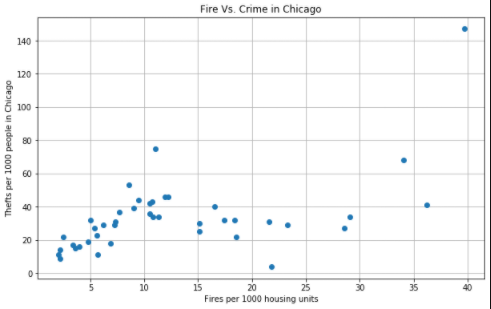
\includegraphics[scale = .85]{CrimeVsHouseFiresPNG.png}\\
As seen, the data show a clear(although not perfect) linear pattern. Next we have gradient descent as a function which takes the parameters $X$,a matrix containing all of the x values of the matrix, $y$, a matrix containing all of the y-values of the dataset, alpha, the learning rate which is $\alpha$ from the previous equation, and $iterations$, which is the number of iterations that gradient descent will perform. The function returns, $costProg$ an array that contains the cost from every iteration of gradient descent, $thetaProg$, an array that contains the value of theta at every iteration of gradient descent, $theta$, the final value of theta and $X$ and $y$ which are the feature and target values of the dataset respectively.\\

    \begin{tcolorbox}[breakable, size=fbox, boxrule=1pt, pad at break*=1mm,colback=cellbackground, colframe=cellborder]
\prompt{In}{incolor}{1}{\boxspacing}
\begin{Verbatim}[commandchars=\\\{\}]
\PY{k}{def} \PY{n+nf}{gradientDescent}\PY{p}{(}\PY{n}{X}\PY{p}{,}\PY{n}{y}\PY{p}{,}\PY{n}{alpha}\PY{p}{,}\PY{n}{iterations}\PY{p}{)}\PY{p}{:}
\PY{c+c1}{\PYZsh{}     initialtheta = np.zeros((X.shape[1],1))}
    \PY{n}{m} \PY{o}{=} \PY{n}{y}\PY{o}{.}\PY{n}{size}
    \PY{n}{X} \PY{o}{=} \PY{n}{X}\PY{o}{.}\PY{n}{reshape}\PY{p}{(}\PY{n}{X}\PY{o}{.}\PY{n}{shape}\PY{p}{[}\PY{l+m+mi}{0}\PY{p}{]}\PY{p}{,}\PY{l+m+mi}{1}\PY{p}{)}
    \PY{n}{y} \PY{o}{=} \PY{n}{y}\PY{o}{.}\PY{n}{reshape}\PY{p}{(}\PY{n}{y}\PY{o}{.}\PY{n}{shape}\PY{p}{[}\PY{l+m+mi}{0}\PY{p}{]}\PY{p}{,}\PY{l+m+mi}{1}\PY{p}{)}
    \PY{n}{X} \PY{o}{=} \PY{n}{np}\PY{o}{.}\PY{n}{insert}\PY{p}{(}\PY{n}{X}\PY{p}{,}\PY{l+m+mi}{0}\PY{p}{,}\PY{l+m+mi}{1}\PY{p}{,}\PY{n}{axis}\PY{o}{=}\PY{l+m+mi}{1}\PY{p}{)}
    \PY{n}{theta} \PY{o}{=} \PY{n}{np}\PY{o}{.}\PY{n}{zeros}\PY{p}{(}\PY{p}{(}\PY{n}{X}\PY{o}{.}\PY{n}{shape}\PY{p}{[}\PY{l+m+mi}{1}\PY{p}{]}\PY{p}{,}\PY{l+m+mi}{1}\PY{p}{)}\PY{p}{)}
    \PY{n}{costProg} \PY{o}{=} \PY{p}{[}\PY{p}{]}
    \PY{n}{thetaProg} \PY{o}{=} \PY{p}{[}\PY{p}{]}
    \PY{k}{for} \PY{n}{i} \PY{o+ow}{in} \PY{n+nb}{range}\PY{p}{(}\PY{n}{iterations}\PY{p}{)}\PY{p}{:}
        \PY{n}{tempTheta} \PY{o}{=} \PY{n}{theta}
        \PY{n}{costProg}\PY{o}{.}\PY{n}{append}\PY{p}{(}\PY{n}{computeCost}\PY{p}{(}\PY{n}{X}\PY{p}{,}\PY{n}{y}\PY{p}{,}\PY{n}{theta}\PY{p}{)}\PY{p}{)}
        \PY{k}{for} \PY{n}{j} \PY{o+ow}{in} \PY{n+nb}{range}\PY{p}{(}\PY{n}{theta}\PY{o}{.}\PY{n}{size}\PY{p}{)}\PY{p}{:}
            \PY{n}{cost} \PY{o}{=} \PY{p}{(}\PY{n}{alpha}\PY{o}{/}\PY{n}{m}\PY{p}{)}\PY{o}{*} \PY{n}{np}\PY{o}{.}\PY{n}{sum}\PY{p}{(}\PY{p}{(}\PY{n}{h}\PY{p}{(}\PY{n}{X}\PY{p}{,}\PY{n}{theta}\PY{p}{)}\PY{o}{\PYZhy{}}\PY{n}{y}\PY{p}{)}\PY{o}{*}\PY{n}{np}\PY{o}{.}\PY{n}{array}\PY{p}{(}\PY{n}{X}\PY{p}{[}\PY{p}{:}\PY{p}{,}\PY{n}{j}\PY{p}{]}\PY{p}{)}\PY{o}{.}\PY{n}{reshape}\PY{p}{(}\PY{n}{m}\PY{p}{,}\PY{l+m+mi}{1}\PY{p}{)}\PY{p}{)}
            \PY{n}{tempTheta}\PY{p}{[}\PY{n}{j}\PY{p}{]} \PY{o}{=} \PY{n}{tempTheta}\PY{p}{[}\PY{n}{j}\PY{p}{]} \PY{o}{\PYZhy{}} \PY{n}{cost}
        \PY{n}{theta} \PY{o}{=} \PY{n}{tempTheta}
        \PY{n}{thetaProg}\PY{o}{.}\PY{n}{append}\PY{p}{(}\PY{n}{theta}\PY{p}{)}
    \PY{k}{return} \PY{n}{costProg}\PY{p}{,}\PY{n}{thetaProg}\PY{p}{,}\PY{n}{theta}\PY{p}{,}\PY{n}{X}\PY{p}{,}\PY{n}{y}
\end{Verbatim}
\end{tcolorbox}
    Now that we have all of our necessary functions defined, we call gradient descent on our data and store the results in the following variables:
    \begin{tcolorbox}[breakable, size=fbox, boxrule=1pt, pad at break*=1mm,colback=cellbackground, colframe=cellborder]
\prompt{In}{incolor}{2}{\boxspacing}
\begin{Verbatim}[commandchars=\\\{\}]
\PY{n}{costProg}\PY{p}{,}\PY{n}{thetaProg}\PY{p}{,}\PY{n}{finTheta}\PY{p}{,}\PY{n}{finX}\PY{p}{,}\PY{n}{finY} \PY{o}{=} \PY{n}{gradientDescent}\PY{p}{(}\PY{n}{features}\PY{p}{,}\PY{n}{targets}\PY{p}{,}\PY{o}{.}\PY{l+m+mi}{001}\PY{p}{,}\PY{l+m+mi}{50}\PY{p}{)}
\end{Verbatim}
\end{tcolorbox}

To show the progression of our theta, we plot the cost of it against the number of iterations. As seen in the following visual, the cost of theta open the first iteration was extremely high. Upon each iteration, as theta became increasingly correct, the cost of theta went down. It is clearly shown that around the tenth iteration, the cost of the model with the updated thetas had essentially converged, meaning that gradient descent had found the optimal values of  theta for the data. 
\begin{tcolorbox}[breakable, size=fbox, boxrule=1pt, pad at break*=1mm,colback=cellbackground, colframe=cellborder]
\prompt{In}{incolor}{3}{\boxspacing}
\begin{Verbatim}[commandchars=\\\{\}]
\PY{n}{plt}\PY{o}{.}\PY{n}{plot}\PY{p}{(}\PY{n+nb}{range}\PY{p}{(}\PY{n+nb}{len}\PY{p}{(}\PY{n}{costProg}\PY{p}{)}\PY{p}{)}\PY{p}{,}\PY{n}{costProg}\PY{p}{,}\PY{l+s+s1}{\PYZsq{}}\PY{l+s+s1}{bo}\PY{l+s+s1}{\PYZsq{}}\PY{p}{)}
\PY{n}{plt}\PY{o}{.}\PY{n}{grid}\PY{p}{(}\PY{k+kc}{True}\PY{p}{)}
\PY{n}{plt}\PY{o}{.}\PY{n}{title}\PY{p}{(}\PY{l+s+s1}{\PYZsq{}}\PY{l+s+s1}{Cost of function vs. iterations}\PY{l+s+s1}{\PYZsq{}}\PY{p}{)}
\PY{n}{plt}\PY{o}{.}\PY{n}{xlabel}\PY{p}{(}\PY{l+s+s1}{\PYZsq{}}\PY{l+s+s1}{Iterations}\PY{l+s+s1}{\PYZsq{}}\PY{p}{)}
\PY{n}{plt}\PY{o}{.}\PY{n}{ylabel}\PY{p}{(}\PY{l+s+s1}{\PYZsq{}}\PY{l+s+s1}{Cost of function}\PY{l+s+s1}{\PYZsq{}}\PY{p}{)}
\PY{n}{plt}\PY{o}{.}\PY{n}{show}\PY{p}{(}\PY{p}{)}
\end{Verbatim}
\end{tcolorbox}

    \begin{center}
    \adjustimage{max size={0.5\linewidth}{0.5\paperheight}}{output_10_0.png}
    \end{center}
    { \hspace*{\fill} \\}
    \begin{tcolorbox}[breakable, size=fbox, boxrule=1pt, pad at break*=1mm,colback=cellbackground, colframe=cellborder]
    Now finally, with the optimal value of theta as found by our gradient descent function, we can plot our model against the data.
\prompt{In}{incolor}{4}{\boxspacing}
\begin{Verbatim}[commandchars=\\\{\}]
\PY{n}{plt}\PY{o}{.}\PY{n}{figure}\PY{p}{(}\PY{n}{figsize} \PY{o}{=} \PY{p}{(}\PY{l+m+mi}{10}\PY{p}{,}\PY{l+m+mi}{6}\PY{p}{)}\PY{p}{)}
\PY{n}{plt}\PY{o}{.}\PY{n}{plot}\PY{p}{(}\PY{n}{xPlot}\PY{p}{,}\PY{n}{finY}\PY{p}{,}\PY{l+s+s1}{\PYZsq{}}\PY{l+s+s1}{o}\PY{l+s+s1}{\PYZsq{}}\PY{p}{)}
\PY{n}{plt}\PY{o}{.}\PY{n}{plot}\PY{p}{(}\PY{n}{xPlot}\PY{p}{,}\PY{n}{finTheta}\PY{p}{[}\PY{l+m+mi}{1}\PY{p}{]}\PY{o}{*}\PY{n}{xPlot}\PY{o}{+}\PY{n}{finTheta}\PY{p}{[}\PY{l+m+mi}{0}\PY{p}{]}\PY{p}{,}\PY{p}{)}
\PY{n}{plt}\PY{o}{.}\PY{n}{xlabel}\PY{p}{(}\PY{l+s+s1}{\PYZsq{}}\PY{l+s+s1}{Fires per 1000 housing units}\PY{l+s+s1}{\PYZsq{}}\PY{p}{)}
\PY{n}{plt}\PY{o}{.}\PY{n}{ylabel}\PY{p}{(}\PY{l+s+s2}{\PYZdq{}}\PY{l+s+s2}{Thefts per 1000 people in Chicago}\PY{l+s+s2}{\PYZdq{}}\PY{p}{)}
\PY{n}{plt}\PY{o}{.}\PY{n}{title}\PY{p}{(}\PY{l+s+s2}{\PYZdq{}}\PY{l+s+s2}{Fire Vs. Crime in Chicago}\PY{l+s+s2}{\PYZdq{}}\PY{p}{)}
\PY{n}{plt}\PY{o}{.}\PY{n}{grid}\PY{p}{(}\PY{k+kc}{True}\PY{p}{)}
\PY{n}{plt}\PY{o}{.}\PY{n}{show}\PY{p}{(}\PY{p}{)}
\end{Verbatim}
\end{tcolorbox}

    \begin{center}
    \adjustimage{max size={0.6\linewidth}{0.6\paperheight}}{output_9_0.png}
    \end{center}
    { \hspace*{\fill} \\}
    
    

\section{Proofs}
\begin{enumerate}
    \item \textbf{Proof that the Cost Function for Univariate Linear Regression is convex}\\
    \medskip Let the cost function be defined by: \[
    J(\theta_0,\theta_1) = \frac{1}{m} \sum_{i = 1}^{m}(h_{\theta}(x_{i})-y_{i})^{2}
    \]
    \textbf{Definitions}\\
    For all $m$ $\in \mathbb{N}$, let $A$ be an arbitrary function where \smallskip $A = \{ (x_1, y_1), (x_2, y_2) \dots (x_m, y_m) \}$.\\
    \smallskip Note that set $A$ represents the number of points in the given data set.\\
    \smallskip Let $h_{\theta}$ be the linear function that we are trying to compute the cost of.\\
    \smallskip $h_{\theta}(x)$ = $\theta_0 + \theta_1x$ where $\theta_0$ is the y-intercept and $\theta_1$ is the slope.\newline
    \textbf{Proof:} Let $x_i \in \mathbb R^n$ be the $i$th training example, let $X$ be a matrix with its $i$th row denoted as $x_i^T$, and let $y$ be a column vector with its $i$th entry denoted as $y_i$.\newline
    For $J:\mathbb{R}^n\rightarrow\mathbb{R}$,
    \begin{align*}
        J(\theta) &= \frac{1}{2m} \sum_{i=0}^m (x_i^T \theta - y_i)^2\\
        &=\frac{1}{2m} \| X \theta - y \|_2^2
    \end{align*}
    For a twice differentiable function, $f$, with $n\in\mathbb{N}$ inputs, let its Hessian matrix be defined as
    \begin{center}
        \begin{bmatrix} 
        \frac{\partial^2 f}{\partial x_1^2} & \frac{\partial^2 f}{\partial x_1\partial x_2} & \dots & \frac{\partial^2 f}{\partial x_1\partial x_n} \\ 
        \frac{\partial^2 f}{\partial x_2\partial x_1} & \frac{\partial^2 f}{\partial x_2^2} & \dots & \frac{\partial^2 f}{\partial x_2\partial x_n} \\ 
        \vdots & \vdots & \ddots & \vdots \\ 
        \frac{\partial^2 f}{\partial x_n\partial x_1} & \frac{\partial^2 f}{\partial x_n\partial x_2} & \dots & \frac{\partial^2 f}{\partial x_n^2} 
        \end{bmatrix}
    \end{center}
    To prove convexity of $f$, its Hessian matrix must be positive definite, or in other words, consist of all positive eigenvalues.\newline
    Given the function, \[f(\theta) = \frac{1}{2m} \| \theta \|_2^2\]
    its Hessian matrix is positive convex, as
    \[\nabla^2 f(\theta) = \frac{1}{m} I\] with $I$ being the identity matrix.\newline
    Thus, we can conclude that the cost function is convex.
    \item \textbf{Proof for the convergence of gradient descent with fixed step size}
    \newline \textbf{Definitions}
    \newline For function f : $\mathbb{R}^d \rightarrow \mathbb{R}$,
    \newline Gradient decent: For an x$_0\in\mathbb{R}^d$ and step size t $\geq$ 0,  gradient descent (GD) refers to the following algorithm : 
    \[
    x_{i+1} = x_{i} - t\nabla f(x_i)
    \]
    Convex: f is convex if for all x, y $\in$ $\mathbb{R}^d$ and 0 $\leq \lambda \leq$ 1,
    \[
    f(\lambda x + (1 - \lambda)y)  \leq  \lambda f(x) + (1 - \lambda)f(y)
    \]
    L-Lipschitz: f is L-Lipschitz if for all x, y $\in$ $\mathbb{R}^d$
    \[
    \norm{\nabla f(x) - \nabla f(y)}_2 \leq \norm{x-y}_2 
    \]
    Let function f be Lipschitz convex, the following properties hold true:
    \newline \textbf{Property 1}: For all x, y $\in$ $\mathbb{R}^d$,
    \[
    f(x) + 	\langle\nabla f(x), y-x\rangle \leq f(y) 
    \]
    \textbf{Property 2}: For all x, y $\in$ $\mathbb{R}^d$, 
    \[
    f(y) \leq f(x) + \langle\nabla f(x), y-x\rangle + \frac{L}{2}\norm{y-x}_2^2
    \]
    \textbf{Property 3}: For y$_1$, y$_2$...y$_k$ $\in$ $\mathbb{R}^d$, 
    \[
    f(\frac{y_1+y_2...+y_k}{k}) \leq \frac{f(y_1)+f(y_2)...+f(y_k)}{k}
    \]
    Now prove that gradient descent converges to a global optimum for Lipschitz convex functions, i.e 
    \newline For a function f that is L-Lipschitz and convex, let x$^*$ be the x at which f(x) is at its minimum, or arg min$_x$f(x). Then for GD with the step size t $\leq$ 1/L: 
    \[
    f(x_k) \leq f(x^*) + \frac{\norm{x_0-x^*}_2^2}{2tk}
    \]
    Proof: 
    \newline Next, we can bound f(x
+), the objective value at the next iteration, in terms of f(x
∗
), the optimal objective
value. Since f is convex, we can write: 
    \begin{equation}
    \begin{split}
    f(x_{i}) + 	\langle\nabla f(x_{i}), x_{i+1}-x_{i}\rangle \leq f(x_{i+1}) 
    \end{split}
    \end{equation}
    \newline Now apply Property 2: 
    \begin{equation}
    \begin{split}
    f(x_{i+1}) & \leq  f(x_{i}) + \langle\nabla f(x_{i}), x_{i+1}-x_{i}\rangle + \frac{L}{2}\norm{x_{i+1}-x_{i}}_2^2 \\
    & = f(x_{i}) + \langle\nabla f(x_{i}), x_{i} - t\nabla f(x_{i})-x_{i}\rangle + \frac{L}{2}\norm{x_{i} - t\nabla f(x_{i})-x_{i}}_2^2 \\
    & = f(x) + \langle\nabla f(x), -t\nabla f(x)\rangle + \frac{L}{2}\norm{- t\nabla f(x_{i})}_2^2 \\
    & = f(x) - t\norm{\nabla f(x_{i})}_2^2 +  \frac{Lt^2}{2}\norm{\nabla f(x_{i})}_2^2 \\
    & = f(x) + t(Lt/2 - 1)\norm{\nabla f(x_{i})}_2^2 \\
    & \leq f(x) + t(L(1/L)/2 - 1)\norm{\nabla f(x_{i})}_2^2 \\
    & = f(x) - \frac{t}{2}\norm{\nabla f(x_{i})}_2^2 \\
    \end{split}
    \end{equation}
\end{enumerate}
\section{Conclusion}
In conclusion, the application of mathematics in machine learning are essential in understanding the conceptual basics of fundamental algorithms. Through this experience, we further expanded our knowledge on machine learning algorithms and their implementations and subsequent applications, while practicing proof writing. Exploring the process by which these equations were derived helped us better grasp the reasons of why they work the way they do and their importance. 
\section{References}


\end{document}